\documentclass{article}

% ---------------------------------------------------------------------------
% Uses the NeurIPS style file. On Overleaf, open the NeurIPS template and
% replace its main .tex with this file (keep the template's neurips_20XX.sty
% and update the package name below to match it).
% ---------------------------------------------------------------------------
\usepackage[preprint]{neurips_2025}

\usepackage[utf8]{inputenc}
\usepackage[T1]{fontenc}
\usepackage{hyperref}
\usepackage{url}
\usepackage{booktabs}
\usepackage{amsfonts,amsmath}
\usepackage{nicefrac}
\usepackage{microtype}
\usepackage{xcolor}
\usepackage{graphicx}

\title{Learning Speed Dating: Bayesian Networks for\\Mutual Attraction}

\author{%
  Author One \\ UC San Diego \\ \texttt{email@ucsd.edu} \And
  Author Two \\ UC San Diego \\ \texttt{email@ucsd.edu}
}

\begin{document}

\maketitle

\begin{abstract}
  % TODO: write once results are in.
  We model the outcome of four-minute speed dates with Bayesian networks
  learned from the Columbia speed-dating experiment. We compare a
  hand-designed network built from our interpretations with networks
  whose structure is learned by the PC algorithm, and evaluate each on
  predicting whether two people both say ``yes.''
\end{abstract}

% ===========================================================================
\section{Problem Description}
\label{sec:problem}

When two strangers meet for a few minutes, what decides whether they want to
see each other again? Our project asks this question in a probabilistic form:
\emph{given what we know about two participants before and during a speed date,
what is the probability that each one wants to see the other again, and which
factors directly affect that decision?} Concretely, for each date we predict the
participant's decision $D \in \{0,1\}$, the partner's decision
$D_o \in \{0,1\}$, and through them the event that the date is a
\emph{match}, $M = D \wedge D_o$. We also want to describe the dependence
structure among the variables that lead to those decisions.

\paragraph{Why it matters.}
Partner choice is one of the most consequential decisions people make, and it is
hard to study because preferences people \emph{state} often differ from the
choices they \emph{reveal}. A speed-dating experiment provides an unusually
structured setting: each participant reports what they look for in a partner,
then has a four-minute date with every participant of the opposite sex in their
session, rates each partner on the same six attributes, and makes a binary
yes/no choice. This lets us
compare stated priorities (e.g.\ how much a person says they care about
intelligence) with the ratings that actually predict a ``yes.'' The same
questions apply to online dating platforms, which rank and recommend millions of
potential matches each day, and more generally to two-sided matching problems
such as hiring, where a pairing succeeds only when \emph{both} sides agree.

\paragraph{Relevance to probabilistic reasoning and learning.}
The problem suits probabilistic graphical models for several reasons.
\begin{itemize}
  \item \textbf{Uncertainty is inherent.} Attraction is noisy: the same
        person may say ``yes'' to one partner and ``no'' to a similar one.
        A model that outputs calibrated probabilities
        $P(D=1 \mid \text{evidence})$ is more useful than a hard
        classifier, and lets us answer queries with any subset of evidence
        (e.g.\ with only pre-date survey answers, or after ratings are seen).
  \item \textbf{Structure is the object of interest.} We care about
        \emph{why} a date succeeds, not only about predicting it. A Bayesian
        network (BN) encodes conditional independencies, so we can ask
        whether, for example, a participant's stated preference for
        attractiveness still matters once we know how attractive they found
        their partner (a $d$-separation question).
  \item \textbf{Knowledge versus data.} We first build a ``natural'' BN by
        hand, grouping the survey variables into interpretable blocks
        (demographics, shared interests, stated preferences, expectations,
        self-perception, the partner's view, and the participant's view of the
        date). We fit its conditional probability tables (CPTs) by maximum
        likelihood, or by EM if we add latent nodes. We then learn a structure
        directly from data with the constraint-based PC algorithm
        \citep{spirtes2000causation} and compare the two, both by held-out
        predictive accuracy and by which edges they share.
  \item \textbf{Stated versus revealed preferences.} Running PC a second time
        on \emph{only} the pre-date survey answers shows how much of the
        outcome can be predicted before two people meet, and how much depends
        on the in-person impression.
\end{itemize}
The data is discrete or easy to discretize, partly missing, and reciprocal
(each date is seen from two sides). These are the issues the course
covers: learning CPTs from counts, handling missing data, discretization, and
learning structure.

% ===========================================================================
\section{Data Sourcing and Processing}
\label{sec:data}

\subsection{Source}

Our data comes from the speed-dating experiment run by
\citet{fisman2006gender} at Columbia Business School between 2002 and 2004
\citep{fisman2006data}. Across 21 sessions (``waves''), 551 graduate and
professional students went on four-minute dates with every participant of the
opposite sex in their session. Session size was not fixed: it ranged from 10 to
44 participants, so a participant had between 5 and 22 dates, and the data
labels each session as a smaller or a larger ``choice'' condition
(\texttt{condtn}). Before the event, each participant filled out a
survey on demographics, hobbies, how important six partner attributes are to
them (attractive, sincere, intelligent, funny, ambitious, shared interests),
and how they rate themselves. In most waves, importance was a budget of 100
points split across the six attributes. In waves 6--9, each attribute instead
got its own 1--10 rating, and the released data rescales these so they also sum
to 100 (see Section~\ref{sec:data}, Preprocessing). After each date they rated the
partner on the same six attributes, gave an overall ``like'' score and an
estimate of how likely the partner was to say yes, and recorded a yes/no
decision.

We use the cleaned version of this data published on Kaggle by
U.~T.~Pedersen \citep{pedersen_kaggle}, which follows the OpenML
\texttt{SpeedDating} release. It has \textbf{8,378 rows and 123 columns}. Each row
is one date seen from one participant's point of view; every date therefore
appears twice, once per side. Partner attributes carry an \texttt{\_o} suffix
(e.g.\ \texttt{attractive\_o} is the partner's rating of the participant), and
the release adds discretized copies of most numeric columns with a
\texttt{d\_} prefix. We also keep the original 195-column Kaggle file
\citep{annavictoria_kaggle} to look up variable definitions.

The labels are reasonably balanced at the individual level:
participants said ``yes'' on 42.0\% of dates
(3,518 of 8,378). Mutual matches are rarer, at 16.5\% (1,380 rows). Gender is
balanced (4,194 male and 4,184 female rows), since every date has one participant of
each sex.

\subsection{Preprocessing}

\paragraph{Decoding and type conversion.}
The OpenML export stores categorical values as Python byte-string literals
(e.g.\ \texttt{b'female'}, \texttt{b'1'}). We strip this encoding, map binary
labels to $\{0,1\}$, and keep the remaining categoricals (gender, race,
field of study) as strings. Missing values appear both as empty cells and as the
token \texttt{b'?'}, and we treat both as missing.

\paragraph{Feature selection.}
We remove columns that are uninformative or that would leak the label:
\begin{itemize}
  \item \texttt{match} is a deterministic function of the two decisions
        ($M = D \wedge D_o$), so it is never used as a feature. We use it
        only to evaluate the match predictions.
  \item \texttt{wave} identifies the session. It carries no information
        about people and would let a model memorize session effects.
  \item \texttt{has\_null} is a dataset bookkeeping flag, and in this export it
        holds the same value in every row.
  \item For the hand-built network we use the discretized hobby
        variables (\texttt{d\_sports}, \ldots, \texttt{d\_yoga}) instead of
        their raw 1--10 versions. We also drop \texttt{interests\_correlate},
        a summary that is computed from the individual hobby scores and is
        therefore redundant with them.
\end{itemize}
The remaining variables are split into seven groups, which become the
blocks of the natural BN: \emph{demographic} (age, age gap, race,
same-race indicator, importance of same race/religion, field),
\emph{shared interests} (17 hobby ratings), \emph{stated preferences}
(the 100-point allocations for self and partner),
\emph{expectations} (expected happiness, expected number of matches),
\emph{self-perception} (self-ratings on five attributes), \emph{partner's
perception} (the partner's stated preferences and ratings of the participant),
and \emph{perception of the date} (the participant's ratings of the partner,
overall like, and guessed probability of being liked).

\paragraph{Discretization.}
We fit tabular CPTs, so every variable must be discrete. Without binning, a
single CPT over several 1--10 or 0--100 parents would have far more entries
than we have rows. We use the three-level bins that come with the
dataset (the \texttt{d\_} columns). Ratings on a 1--10 scale are binned into
$[0\text{--}5]$, $[6\text{--}8]$, $[9\text{--}10]$, and 100-point
importance allocations into $[0\text{--}15]$, $[16\text{--}20]$, $[21\text{--}100]$.
For example, \texttt{d\_like} has 2,944 / 4,827 / 607 rows in its three bins.

The importance allocations need extra care. Within one person, a point is
worth the same on every attribute, but the six values always add up to 100, so
they are not independent. Giving more weight to one attribute means giving less
to the others, which builds negative correlations into the data before any real
preference effect. This matters for PC, whose independence tests can mistake the
constraint for real dependencies. Because of the shared total, only five of the
six values carry information.
The scale also differs across waves. In waves 6--9 (101 of 542 participants with
answers), the values are 1--10 ratings rescaled to sum to 100. We confirmed this
from the data: every such participant's values are integer 1--10 scores
multiplied by $100/S$, where $S$ is the sum of that person's six scores. These
waves never exceed 28 points on one attribute, while elsewhere participants put
up to 100 points on one. As a result, 66\% of the importance values in waves 6--9
fall in the middle bin ($[16\text{--}20]$), compared with 31\% in other waves.
We therefore treat the scale as a wave-level variable (or drop these
waves) when we fit the importance variables. Nine participants' allocations do
not sum to 100 (range 90--148), and we renormalize them.
Three levels keep the CPTs small: a node with four ternary parents needs
$3^4\cdot 2 = 162$ free parameters, which our data can estimate reliably,
and the bins still separate low, typical and high ratings. Age difference
(\texttt{d\_age}) is already an integer number of years. Its long tail runs up to 37 years,
so we cap it, putting every gap of 7 or more years into one bin. Free-text \texttt{field} has 260 distinct values,
so we either map it to the coarse field codes of the original study or leave
it out of the network.

For methods that need continuous inputs, such as the PCA plot in our
exploratory analysis,
we turn each binned value back into a number by taking the midpoint of its
range (e.g.\ $[6\text{--}8] \mapsto 7$). We then one-hot encode the categorical columns and
standardize every feature to zero mean and unit variance.

\paragraph{Missing data.}
Missing values are common: 57 of the 123 columns contain missing
entries, 18,173 cells in total, and \textbf{87.5\% of rows (7,330) have at least
one missing value}. Dropping every incomplete row would leave too little data, so we
handle columns differently depending on how much is missing:
\begin{itemize}
  \item \texttt{expected\_num\_interested\_in\_me} is missing in 78.5\% of rows
        (it was asked in only a few waves), so we drop it.
  \item The other columns are missing much less often. The worst are
        \texttt{shared\_interests\_o} and \texttt{shared\_interests\_partner}
        at about 13\%, \texttt{expected\_num\_matches} at 14\%, and
        the remaining ratings at under 9\%. For exploratory analysis we fill
        numeric columns with the median and categorical columns with the mode.
  \item For BN parameter learning, single imputation makes the
        CPTs look more certain than they are. We instead treat missing entries as
        unobserved and fit the CPTs with EM, which uses the partly observed
        rows rather than inventing values for them. The same machinery
        also lets us add latent nodes later. As a baseline we also run plain MLE
        on the imputed data, so we can see how much this choice matters.
\end{itemize}

\paragraph{Train/test split.}
We hold out 15\% of the data for testing and learn structure and parameters on
the remaining 85\%. Each date appears twice (once from each side) and each
participant has between 5 and 22 dates, so a random row split would put information
about the same person in both sets. We therefore split by \emph{participant}:
all rows for a given participant go to the same side of the split.

\paragraph{Why these steps matter.}
Each step either keeps the model from learning things it should not or
keeps the learning problem feasible. Removing \texttt{match} and the session
identifier prevents label and session leakage, which would make accuracy look
better than it is. Discretizing to three levels keeps the number of
CPT parameters small enough to estimate from about 7,000 training rows. Handling
missingness with EM rather than dropping rows keeps the 87.5\% of incomplete rows
and avoids skewing the data toward the waves that asked every question.
Splitting by participant makes held-out accuracy a fair estimate of how
the model does on people it has not seen.
Figure~\ref{fig:pca} projects the processed features onto their first two
principal components. The three outcomes (neither yes, one yes, match) overlap
heavily, so no single linear direction separates them. This supports using a
model that reasons over the joint distribution of many variables.

\begin{figure}[t]
  \centering
  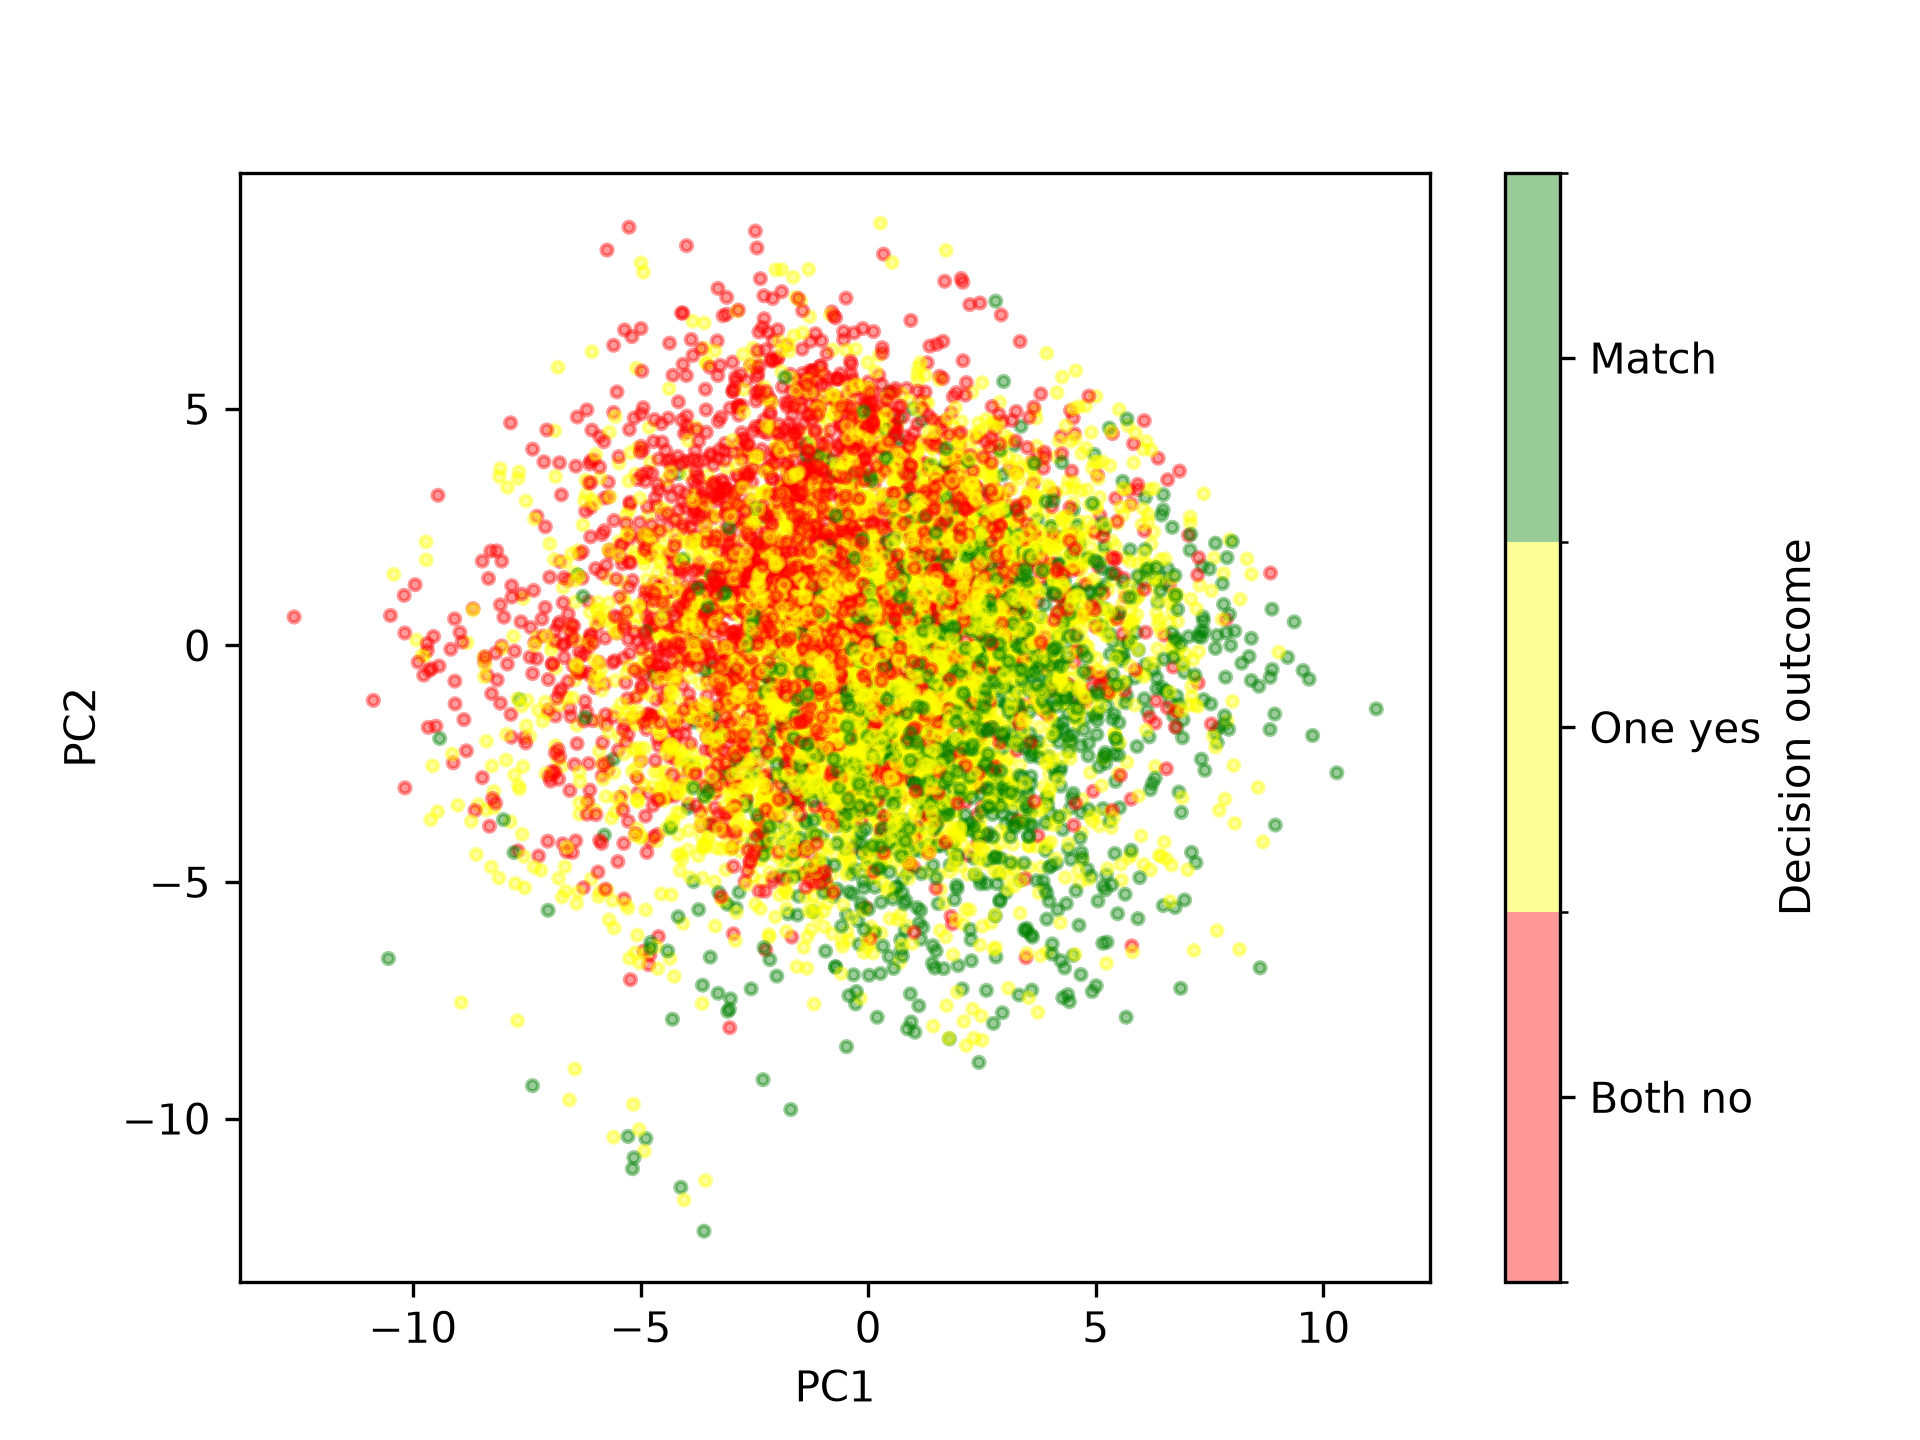
\includegraphics[width=0.6\linewidth]{../figures/PCA_colored.png}
  \caption{First two principal components of the standardized, imputed features,
  colored by outcome. The outcome classes overlap heavily in this projection.}
  \label{fig:pca}
\end{figure}

% ===========================================================================
\section{Methodology}
\label{sec:method}
% TODO

\section{Results}
\label{sec:results}
% TODO

\section{Discussion}
\label{sec:discussion}
% TODO

\section{Conclusion}
\label{sec:conclusion}
% TODO

\bibliographystyle{plainnat}
\bibliography{references}

\end{document}
